\documentclass[english,]{IEEEtran}
\usepackage{lmodern}
\usepackage{amssymb,amsmath}
\usepackage{ifxetex,ifluatex}
\usepackage{fixltx2e} % provides \textsubscript
\ifnum 0\ifxetex 1\fi\ifluatex 1\fi=0 % if pdftex
  \usepackage[T1]{fontenc}
  \usepackage[utf8]{inputenc}
\else % if luatex or xelatex
  \ifxetex
    \usepackage{mathspec}
  \else
    \usepackage{fontspec}
  \fi
  \defaultfontfeatures{Ligatures=TeX,Scale=MatchLowercase}
\fi
% use upquote if available, for straight quotes in verbatim environments
\IfFileExists{upquote.sty}{\usepackage{upquote}}{}
% use microtype if available
\IfFileExists{microtype.sty}{%
\usepackage{microtype}
\UseMicrotypeSet[protrusion]{basicmath} % disable protrusion for tt fonts
}{}
\usepackage[unicode=true]{hyperref}
\hypersetup{
            pdftitle={A Survey of Techniques for Price Stabilisation of Cryptocurrencies},
            pdfkeywords={Stablecoin, Blockchain, Cryptocurrencies},
            pdfborder={0 0 0},
            breaklinks=true}
\urlstyle{same}  % don't use monospace font for urls
\ifnum 0\ifxetex 1\fi\ifluatex 1\fi=0 % if pdftex
  \usepackage[shorthands=off,main=english]{babel}
\else
  \usepackage{polyglossia}
  \setmainlanguage[]{english}
\fi
\usepackage{longtable,supertabular,booktabs}
% Fix footnotes in tables (requires footnote package)
\IfFileExists{footnote.sty}{\usepackage{footnote}\makesavenoteenv{long table}}{}
\usepackage{graphicx,grffile}
\makeatletter
\def\maxwidth{\ifdim\Gin@nat@width>\linewidth\linewidth\else\Gin@nat@width\fi}
\def\maxheight{\ifdim\Gin@nat@height>\textheight\textheight\else\Gin@nat@height\fi}
\makeatother
% Scale images if necessary, so that they will not overflow the page
% margins by default, and it is still possible to overwrite the defaults
% using explicit options in \includegraphics[width, height, ...]{}
\setkeys{Gin}{width=0.8\maxwidth,height=0.8\maxheight,keepaspectratio}
\IfFileExists{parskip.sty}{%
\usepackage{parskip}
}{% else
\setlength{\parindent}{0pt}
\setlength{\parskip}{6pt plus 2pt minus 1pt}
}
\setlength{\emergencystretch}{3em}  % prevent overfull lines
\providecommand{\tightlist}{%
  \setlength{\itemsep}{0pt}\setlength{\parskip}{0pt}}
\setcounter{secnumdepth}{5}
% Redefines (sub)paragraphs to behave more like sections
\ifx\paragraph\undefined\else
\let\oldparagraph\paragraph
\renewcommand{\paragraph}[1]{\oldparagraph{#1}\mbox{}}
\fi
\ifx\subparagraph\undefined\else
\let\oldsubparagraph\subparagraph
\renewcommand{\subparagraph}[1]{\oldsubparagraph{#1}\mbox{}}
\fi

% set default figure placement to htbp
\makeatletter
\def\fps@figure{htbp}
\makeatother

\makeatletter
\let\oldlt\longtable
\let\endoldlt\endlongtable
\def\longtable{\@ifnextchar[\longtable@i \longtable@ii}
\def\longtable@i[#1]{\begin{figure}[t]
\onecolumn
\begin{minipage}{0.5\textwidth}
\oldlt[#1]
}
\def\longtable@ii{\begin{figure}[t]
\onecolumn
\begin{minipage}{0.5\textwidth}
\oldlt
}
\def\endlongtable{\endoldlt
\end{minipage}
\twocolumn
\end{figure}}
\makeatother

\title{A Survey of Techniques for Price Stabilisation of Cryptocurrencies}

\author{
            \IEEEauthorblockN{Robert Wessel Blokzijl}
        \IEEEauthorblockA{%
            TU Delft \\
            Delft, The Netherlands \\
            R.W.Blokzijl@student.tudelft.nl}
        }

\date{\today}

\begin{document}
\maketitle
\begin{abstract}
Stablecoins are hot in the crypto space. With the 5th largest
cryptocurrency and stablecoin Tether, now the subject of a trillion
dollar lawsuit, many look to other stablecoins as a safe store of value.
The techniques used by these coins vary massively. This survey discusses
techniques used by the largest and most promising stablecoins to hold a
stable value.
\end{abstract}

\begin{IEEEkeywords}
    Stablecoin;
    Blockchain;
    Cryptocurrencies\end{IEEEkeywords}

\hypertarget{introduction}{%
\section{Introduction}\label{introduction}}

Centralisation, non-transparency and a trillion dollar lawsuit would
normally lead to crypto investors avoiding you like the plague. For
Tether however it lead to a market cap of over 4 Billion dollars. With
Tether currently being the most the most traded cryptocurrency despite
its controversies we are left to wonder what makes a coin that trades at
1 dollar so attractive to investors.

Cryptocurrencies have so far been notoriously volatile in price. Making
the assets unsuited for both investments in the long term, and payments
in the short term.

Another need for price-stable currencies exists among crypto traders.
When the crypto-markets decrease in value, the entire market tends move
as a whole. In this case traders want to move their assets out of the
volatile ``new world'' assets and into traditional currencies like the
Dollar to wait out de dip in de market. However these transactions are
limited by the speed of the old payment networks. A coin that is stable
with respect to the US Dollar would solve this problem by allowing
traders to change positions between the Dollar and crypto currencies in
a quick, decentralised{[}1{]} and programmable {[}2{]} way.

With Tether having proves the need for a stablecoin, many
cryptocurrencies have followed, some solving problems of those who have
come before. MakerDAOs DAI {[}3{]}, currently the 5th biggest stablecoin
and the 52th biggest cryptocurrency with a market cap of 103 million
USD, aims to be a fully decentralised stablecoin that maintains a value
of 1 USD. Dai provides a coin that enables distributed peer-to-peer
lending with the stability of the Dollar while having no centralised
component.

\begin{figure}
\centering
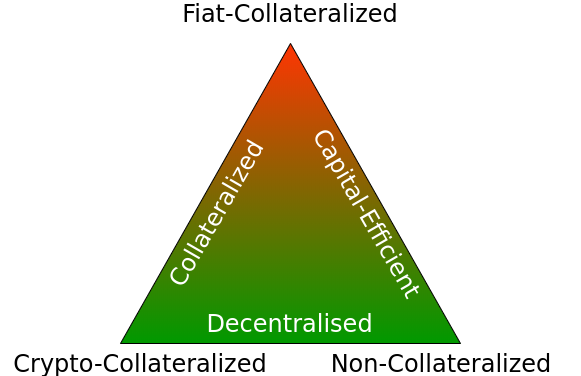
\includegraphics{img/Triangle.png}
\caption{Inherent trade-offs of stablecoins \label{triangle_label}}
\end{figure}

\begin{figure}
\centering
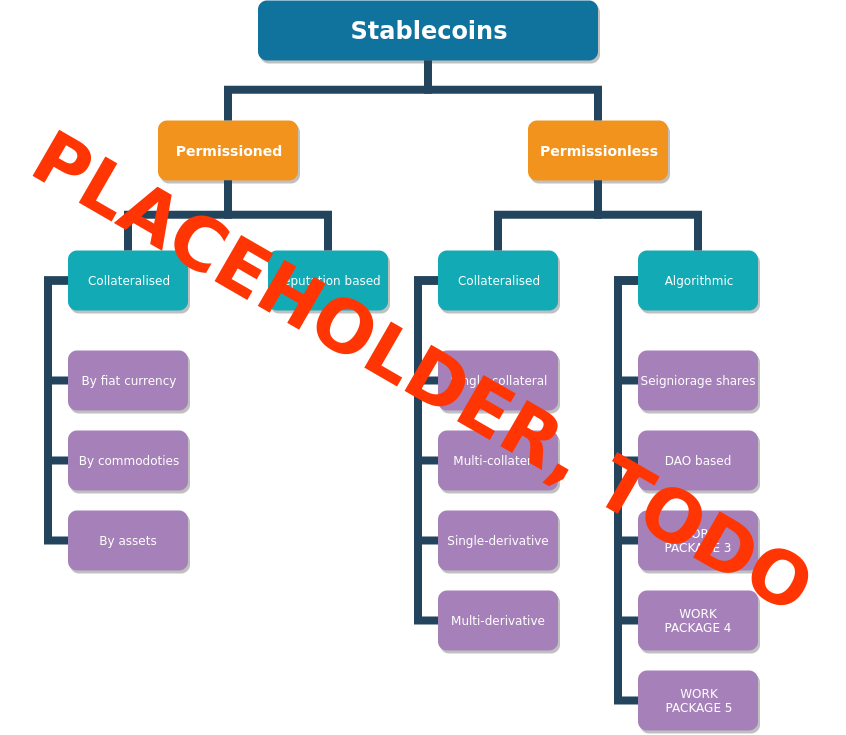
\includegraphics{img/intro.png}
\caption{Taxonomy of stablecoins \label{intro_label}}
\end{figure}

MakerDAO is part of a bigger movement. The Decentralised Finance
movement is an open community of decentralised financial platforms that
aims to revolutionise the financial world by replacing many of the
worlds financial systems. Within this project there are a number of
stablecoins and other tokens that are pegged to real world assets that
use decentralised techniques for providing financial derivatives.

This survey presents a history of the significant stablecoins and pegged
assets invented so far, and classifies and generalises the techniques
that are common among them.

First we discuss the topic of the purpose of money, the meaning of value
and stability, and some currency pegs used in our traditional monetary
system in Chapter 2. We then describe the simplest and most successful
stablecoins, namely the centralised coins in Chapter 3. In Chapter 4 we
go into the more complex topic of decentralised assets and their methods
for maintaining pegs to real world assets without a central party
guaranteeing the peg. We then go deeper into the theory in Chapter 5
where we look at the research into the viability of stablecoins. We then
end with a discussion of the research on stablecoins in Chapter 6 and a
conclusion of the survey in Chapter 7.

\hypertarget{background}{%
\section{Background}\label{background}}

Before we get to the techniques used for stabilisation some concepts and
terms need to be defined. In this chapter we define the purpose and
requirements of money. We define what it means for a currency to be
stable, and what it means for a currency to be collateralized.

\hypertarget{the-purpose-of-money-and-the-requirements-of-a-stablecoin}{%
\subsection{The purpose of money and the requirements of a
stablecoin}\label{the-purpose-of-money-and-the-requirements-of-a-stablecoin}}

In ``On the Origin of Money'' {[}4{]} Karl Menger describes how people
settle on a currency as a method of exchange. He describes that the
willingness of people to exchange their goods for a commodity depends:

\begin{enumerate}
\def\labelenumi{\arabic{enumi}.}
\tightlist
\item
  Upon their ability to trade it for goods (demand)
\item
  Upon the scarcity of the commodity (supply)
\item
  Upon the divisibility, durability and practicality of the commodity.
\item
  Upon the development of the market, and of speculation in particular.
\item
  Upon the limitations imposed politically and socially upon exchange,
  consumption and transfer from one period of time to another
\end{enumerate}

\hypertarget{the-meaning-of-value-and-stability}{%
\subsection{The meaning of value and
stability,}\label{the-meaning-of-value-and-stability}}

An certain configuration of these factors is required for a stable store
of value, and need to be controlled by some mechanism in order to
maintain a stable price of the commodity.

In the value of money {[}5{]} Pigou describes the role of the money
supply in the Quantity theory of money and its relation to the price.
The quantity theory of money states:

\[ M \times V = P \times T \]

Where \(M\) is the money supply, \(V\) is the velocity of circulation,
\(P\) is the price of the coin and \(T\) are all transactions done with
the currency.

This implies that the price of a currency can be controlled by
increasing and decreasing the money supply. Indeed this is a technique
also currently used by central to prevent deflation of their currencies.

In this survey we will see currencies vary both \(M\) and \(V\) as a
means to keep \(P\) at a stable level.

\hypertarget{making-a-market}{%
\subsection{Making a market}\label{making-a-market}}

The easiest way to keep a currency stable is to simply have it derive
its value from a different asset that already has the desired stability.
This is called pegging.

The pegging of a token to an asset can be achieved by allowing investors
to trade the token for the asset at any time. Note that a this may
involve the trade of a secondary asset as intermediary store of value.

The first pegs were tracking the value of gold. Every unit of a currency
could be exchanged for a certain amount of gold. As described in ``The
Gold Standard'' {[}6{]} by Cooper, the US dollar has been pegged to Gold
for some of its years to maintain the confidence of the public.

The most common way to guarantee an exchange rate is to hold some form
of collateral. The most obvious collateral for the token, is the asset
it is pegged to, but this can also be another commodity that can be
traded for the asset at any time. Of course this requires some
guarantees or assumptions about the price stability of this commodity to
ensure that all outstanding tokens can be redeemed. If the amount of
collateral, or the value of the collateral, is such that less that 100\%
of tokens can be redeemed for the original asset, the token is
considered under-collateralized. This can have large ramifications to
investor trust, and might thus undermine the stability of the coin and
the viability of the network.

Any entity or system that facilitates the exchange of the token for the
collateral is called a market maker. In this survey two main categories
of market makers will make an appearance, centralised organisations and
decentralised systems.

\hypertarget{stabilisation-by-centralisation}{%
\section{Stabilisation by
Centralisation}\label{stabilisation-by-centralisation}}

With more control over the supply of a currency, the price stabilisation
of a currency is significantly simplified. Minting more in times of high
demand, though looked down upon, is a powerful way of controlling the
value of a currency and preventing runaway deflation. Conversely,
reducing the rate of minting slows down inflation of the currency.

Another way of stabilising a currency is to peg it to an already
existing currency or commodity. This method brings with it questions
about collateralization, transparency, risk, and the meaning of value.

In this section we explore the techniques employed by both central
reserve, and pegged stablecoins.

\hypertarget{the-reserve-bank-stablecoin}{%
\subsection{The reserve bank
stablecoin}\label{the-reserve-bank-stablecoin}}

Combining the proven success of central banks with the benefits of fast
payment systems {[}7{]}, organisations like JPMorgan {[}8{]} and the
Libra Association {[}9{]} aim to create a stable currency by using their
reputation as established financial institutions. So far, no coin has
managed to be stable off of its reputation alone, and whether this will
ever happen is yet to be seen.

\hypertarget{pegged-by-currency-reserves}{%
\subsection{Pegged by currency
reserves}\label{pegged-by-currency-reserves}}

Since stabilisation by reputation is often not good enough for investors
looking for a safe store of value, a stablecoin with stringer guarantees
about its future value is needed. The simplest way to do this is to
simply peg the cryptocurrency to another currency and guaranteeing a 1:1
exchange rate by holding enough collateral in order to make any investor
whole at any time in the future.

\begin{figure}
\centering
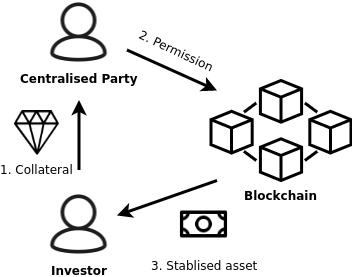
\includegraphics{img/Centralised_create.png}
\caption{Minting a pegged crypto-asset \label{cent_create_label}}
\end{figure}

Figure \ref{cent_create_label} describes the general way in which pegged
crypto assets are created. The centralised party in the image provides
some guarantee about the exchange rate. For this example we assume a peg
for 1 stabilised asset to always be worth 1 dollar. In this context, the
dollar is provided as collateral for the asset in the following way.

\begin{enumerate}
\def\labelenumi{\arabic{enumi}.}
\tightlist
\item
  1 dollar is transferred from the investor to the centralised party
  using traditional payment systems.
\item
  The centralised party mints 1 stabilised asset and transfers it to the
  investor
\item
  The investor is free to use the asset as they please
\end{enumerate}

\begin{figure}
\centering
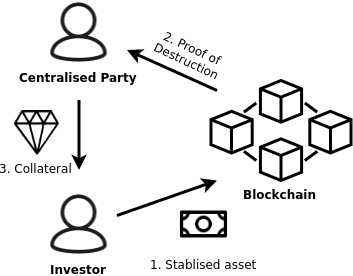
\includegraphics{img/Centralised_destroy.png}
\caption{Burning a pegged-crypto asset \label{cent_destoy_label}}
\end{figure}

Figure \ref{cent_destoy_label} illustrates the general way in which
pegged crypto assets can be traded back for the original asset.

\begin{enumerate}
\def\labelenumi{\arabic{enumi}.}
\setcounter{enumi}{-1}
\tightlist
\item
  Anyone can obtain the stabilised asset by trading for it on some
  market or by having one minted by the centralised party.
\item
  Any investor who holds a stabilised asset can send it to the
  blockchain to be burned.
\item
  Upon receiving a proof of destruction, the centralised party will send
  an equivalent amount of dollars back to the investor.
\item
  The investor is now out of their position.
\end{enumerate}

By guaranteeing that there is always a 1:1 exchange rate between the
collateral and the stabilised asset, the asset is pegged at a 1:1 ratio
even in external markets. This illustrated using the following two
scenarios.

When the stabilised asset trades for more than 1 dollar on the open
market, anyone can make an instant profit by minting more assets, and
immediately selling them on the open market. This process will continue
to increase the supply of the asset until the price is back down to 1
dollar.

Conversely, when the stabilised asset trades for less than 1 dollar on
the open market, anyone can make an instant profit by buying the coins
on the open market, and immediately burning them. This process will
continue to decrease the supply of the asset until the price is back up
to 1 dollar.

\hypertarget{benefits-of-centralisation}{%
\subsubsection{Benefits of
Centralisation}\label{benefits-of-centralisation}}

Like illustrated in figure \ref{triangle_label}, fiat-collateralized
pegs can not be maintained by a fully decentralised system. The limiting
factor is the fact that fiat-currencies need to be held by some party.

Some argue the price guarantees of pegging to a fiat-currency outweighs
the sacrifice of decentralisation. The success of currencies like Tether
{[}10{]}, Centres USDC {[}11{]}, PAXos {[}12{]}, and TrueUSD{[}13{]}
illustrate this with their combined market capitalization of 5 Billion
USD.

\hypertarget{critiques-of-centralisation-and-solutions}{%
\subsubsection{Critiques of Centralisation and
solutions}\label{critiques-of-centralisation-and-solutions}}

It goes without saying that having a centralised storage of anything
creates a central point of failure and control. Since trust in the
crypto space has long been based on what is verifiable, proving the
absence of fraud becomes a new challenge. To address the concerns of
coin holders the different stablecoin market makers provide different
guarantees with respect to the proper storage of collateral. Common ways
to improve investor confidence include:

\begin{enumerate}
\def\labelenumi{\arabic{enumi}.}
\tightlist
\item
  Regular audits providing proof of collateral (Tether {[}10{]}, USDC
  {[}11{]}, PAXos {[}12{]}, TrueUSD {[}13{]})
\item
  Multiple independent collateral trust accounts (TrueUSD
  {[}TrueUSD:whitepaper{]}, Stasis Euro {[}14{]})
\item
  Subjecting themselves to established regulations and providing FDIC-
  insurance. (PAXos {[}12{]})
\end{enumerate}

Through these means stablecoin organisations aim to counteract the lack
of transparency and the risk of under-collateralization.

\hypertarget{expansions-on-fiat-currency-pegging}{%
\subsubsection{Expansions on fiat-currency
pegging}\label{expansions-on-fiat-currency-pegging}}

Essentially, a centralised currency-pegged stablecoin is just a
tokenised fiat-currency. This concept can be expanded to more than just
traditional currencies. Using tokenisation and central storage it is
possible to peg the value of a crypto coin to anything that has value in
the real world. As such some stablecoins peg their value to the original
form of money: Gold. Today, stablecoins like PAX Gold {[}15{]} and
DigixDAO {[}16{]} hold gold in trust for their crypto holders. Though
the gold provides a strong guarantee that the stablecoin will hold its
value, the coins are still less stable than the Dollar as there is no
central agency stabilising gold.

Expanding even further on the concept of tokenised assets as
stablecoins, any collection of assets that is stable on average can
provide a stablecoin. Even though the US Dollar is seen as the most
stable currency world-wide, it is still dependent on the stability of
the United States economy. To address this stablecoins like Globcoin
{[}17{]} and x8currency {[}18{]} aim to create an asset that tracks
multiple currencies as well as gold. Thus creating a coin that is ``more
stable'' than the US Dollar. Whether these coins will ever have a
mainstream appeal is impossible to predict, but the theoretical value of
having a globally stable coin is hard to dispute.

\hypertarget{overview-of-the-largest-stablecoins}{%
\subsubsection{Overview of the largest
stablecoins}\label{overview-of-the-largest-stablecoins}}

To provide a glimpse of the usage of the techniques described in this
chapter the table \ref{TODO} describes the 8 central stablecoins with
the highest market capitalisation and some of their operational aspects:

\begin{table*}[t]\begin{center}\begin{supertabular}[]{@{}lllllll@{}}
\toprule
\begin{minipage}[b]{0.14\textwidth}\raggedright
Stablecoin\strut
\end{minipage} & \begin{minipage}[b]{0.08\textwidth}\raggedright
Market Cap\strut
\end{minipage} & \begin{minipage}[b]{0.07\textwidth}\raggedright
Pegged asset\strut
\end{minipage} & \begin{minipage}[b]{0.10\textwidth}\raggedright
Escrow\strut
\end{minipage} & \begin{minipage}[b]{0.07\textwidth}\raggedright
FDIC-insurance\strut
\end{minipage} & \begin{minipage}[b]{0.04\textwidth}\raggedright
Launch\strut
\end{minipage} & \begin{minipage}[b]{0.30\textwidth}\raggedright
Notes\strut
\end{minipage}\tabularnewline
\midrule
\begin{minipage}[t]{0.14\textwidth}\raggedright
Tether{[}10{]}\strut
\end{minipage} & \begin{minipage}[t]{0.08\textwidth}\raggedright
4 Billion USD\strut
\end{minipage} & \begin{minipage}[t]{0.07\textwidth}\raggedright
USD\strut
\end{minipage} & \begin{minipage}[t]{0.10\textwidth}\raggedright
Single organisation\strut
\end{minipage} & \begin{minipage}[t]{0.07\textwidth}\raggedright
No\strut
\end{minipage} & \begin{minipage}[t]{0.04\textwidth}\raggedright
2014\strut
\end{minipage} & \begin{minipage}[t]{0.30\textwidth}\raggedright
Largest Stablecoin, 4th largest cryptocurrency\strut
\end{minipage}\tabularnewline
\begin{minipage}[t]{0.14\textwidth}\raggedright
USDC{[}11{]}\strut
\end{minipage} & \begin{minipage}[t]{0.08\textwidth}\raggedright
464 Million USD\strut
\end{minipage} & \begin{minipage}[t]{0.07\textwidth}\raggedright
USD\strut
\end{minipage} & \begin{minipage}[t]{0.10\textwidth}\raggedright
Single organisation\strut
\end{minipage} & \begin{minipage}[t]{0.07\textwidth}\raggedright
Some exchanges\strut
\end{minipage} & \begin{minipage}[t]{0.04\textwidth}\raggedright
2018\strut
\end{minipage} & \begin{minipage}[t]{0.30\textwidth}\raggedright
Created and owned by various crypto exchanges\strut
\end{minipage}\tabularnewline
\begin{minipage}[t]{0.14\textwidth}\raggedright
PAXos{[}12{]}\strut
\end{minipage} & \begin{minipage}[t]{0.08\textwidth}\raggedright
238 Million USD\strut
\end{minipage} & \begin{minipage}[t]{0.07\textwidth}\raggedright
USD\strut
\end{minipage} & \begin{minipage}[t]{0.10\textwidth}\raggedright
Single organisation\strut
\end{minipage} & \begin{minipage}[t]{0.07\textwidth}\raggedright
Yes\strut
\end{minipage} & \begin{minipage}[t]{0.04\textwidth}\raggedright
2018\strut
\end{minipage} & \begin{minipage}[t]{0.30\textwidth}\raggedright
Regulated by the New York State Department of Financial Services\strut
\end{minipage}\tabularnewline
\begin{minipage}[t]{0.14\textwidth}\raggedright
TrueUSD{[}13{]}\strut
\end{minipage} & \begin{minipage}[t]{0.08\textwidth}\raggedright
161 Million USD\strut
\end{minipage} & \begin{minipage}[t]{0.07\textwidth}\raggedright
USD\strut
\end{minipage} & \begin{minipage}[t]{0.10\textwidth}\raggedright
Multiple independent\strut
\end{minipage} & \begin{minipage}[t]{0.07\textwidth}\raggedright
Some escrows\strut
\end{minipage} & \begin{minipage}[t]{0.04\textwidth}\raggedright
2018\strut
\end{minipage} & \begin{minipage}[t]{0.30\textwidth}\raggedright
Distributes risk with multiple independent escrows\strut
\end{minipage}\tabularnewline
\begin{minipage}[t]{0.14\textwidth}\raggedright
Stasis{[}14{]}\strut
\end{minipage} & \begin{minipage}[t]{0.08\textwidth}\raggedright
35 Million USD\strut
\end{minipage} & \begin{minipage}[t]{0.07\textwidth}\raggedright
Euro\strut
\end{minipage} & \begin{minipage}[t]{0.10\textwidth}\raggedright
Multiple independent\strut
\end{minipage} & \begin{minipage}[t]{0.07\textwidth}\raggedright
No\strut
\end{minipage} & \begin{minipage}[t]{0.04\textwidth}\raggedright
2018\strut
\end{minipage} & \begin{minipage}[t]{0.30\textwidth}\raggedright
Largest Euro Stablecoin\strut
\end{minipage}\tabularnewline
\begin{minipage}[t]{0.14\textwidth}\raggedright
BUSD{[}12{]}\strut
\end{minipage} & \begin{minipage}[t]{0.08\textwidth}\raggedright
18 Million USD\strut
\end{minipage} & \begin{minipage}[t]{0.07\textwidth}\raggedright
USD\strut
\end{minipage} & \begin{minipage}[t]{0.10\textwidth}\raggedright
Single organisation\strut
\end{minipage} & \begin{minipage}[t]{0.07\textwidth}\raggedright
Yes\strut
\end{minipage} & \begin{minipage}[t]{0.04\textwidth}\raggedright
2019\strut
\end{minipage} & \begin{minipage}[t]{0.30\textwidth}\raggedright
Issued by PAXos for the Binance exchange\strut
\end{minipage}\tabularnewline
\begin{minipage}[t]{0.14\textwidth}\raggedright
USDK\strut
\end{minipage} & \begin{minipage}[t]{0.08\textwidth}\raggedright
28 Million USD\strut
\end{minipage} & \begin{minipage}[t]{0.07\textwidth}\raggedright
USD\strut
\end{minipage} & \begin{minipage}[t]{0.10\textwidth}\raggedright
Single organisation\strut
\end{minipage} & \begin{minipage}[t]{0.07\textwidth}\raggedright
No\strut
\end{minipage} & \begin{minipage}[t]{0.04\textwidth}\raggedright
2019\strut
\end{minipage} & \begin{minipage}[t]{0.30\textwidth}\raggedright
Owned and operated by the oklink exchange\strut
\end{minipage}\tabularnewline
\begin{minipage}[t]{0.14\textwidth}\raggedright
PAX Gold{[}15{]}\strut
\end{minipage} & \begin{minipage}[t]{0.08\textwidth}\raggedright
12 Million USD\strut
\end{minipage} & \begin{minipage}[t]{0.07\textwidth}\raggedright
Gold (1 ounce)\strut
\end{minipage} & \begin{minipage}[t]{0.10\textwidth}\raggedright
Single organisation\strut
\end{minipage} & \begin{minipage}[t]{0.07\textwidth}\raggedright
No\strut
\end{minipage} & \begin{minipage}[t]{0.04\textwidth}\raggedright
2019\strut
\end{minipage} & \begin{minipage}[t]{0.30\textwidth}\raggedright
Gold held in custody by PAXos Trust Company\strut
\end{minipage}\tabularnewline
\bottomrule
\tabularnewline
\end{supertabular}
\caption{TODO \label{TODO}}
\end{center}\end{table*}

Some interesting observations can be made from the table.

\begin{enumerate}
\def\labelenumi{\arabic{enumi}.}
\tightlist
\item
  The PAXos company operates 3 of the top 8 stablecoins.
\item
  3 of the top 8 stablecoins are operated by exchanges including the
  second largest stablecoin USDC.
\item
  Gold based stablecoins still make up a small portion of the market
  with PAX Gold being the largest with a market cap of 12 million.
\end{enumerate}

\hypertarget{stabilised-while-decentralised}{%
\section{Stabilised while
Decentralised}\label{stabilised-while-decentralised}}

Though many centralised stablecoins are becoming more diversified in
their collateralization, the organisations that run them remain a
central point of failure. The risk of collateral depletion by market
maker failure is always prevalent and though some stablecoins store
their collateral with bankruptcy remote companies, this just moves the
risk to a different central entity.

To protect investors from the failure of any central entity and even the
failure of the financial system as a whole, new stablecoins have emerged
that remain price-stable in a decentralised manner. These coins come in
two main categories:

\begin{enumerate}
\def\labelenumi{\arabic{enumi}.}
\tightlist
\item
  Crypto-Collateralized Stablecoins
\item
  Algorithmic Stablecoins
\end{enumerate}

This section explains the mechanisms that keep these coins stable,
provides a comparison of their advantages and disadvantages, and a
general overview of the largest decentralised stablecoins on the market
right now in each category.

\hypertarget{crypto-collateralized-stablecoins}{%
\subsection{Crypto-Collateralized
Stablecoins}\label{crypto-collateralized-stablecoins}}

The success of the centralised stablecoins shows that the backing of a
stablecoin with 100\% collateral is a reliable way to keep a currency
price stable.

The main problem with backing a decentralised stablecoin with some type
of collateral is that there needs to be a mechanism of exchange between
the stablecoin and the collateral. When the collateral is fiat-currency
or some real world asset, there must always be a central party that
holds the collateral and facilitates the mechanism of exchange.

Crypto-collateralized coins build on the idea that a holder of a
stablecoin can always get their share of the collateral back, but in a
fully automated and decentralised manner.

Crypto-collateral coins allow the exchange of the pegged currency such
that even the organisation that created the stablecoin has no power over
the collateral. Initially it may seem like we need a collateral with the
following requirements:

\begin{enumerate}
\def\labelenumi{\arabic{enumi}.}
\tightlist
\item
  Stable - to stabilise the stablecoin
\item
  Decentralised - to avoid central control
\item
  Fully programmable - to automate the collateral exchange mechanism
\end{enumerate}

The problem here is quite obvious, we are looking for precisely the
thing we are trying to create, a decentralised stablecoin. In order to
solve this, crypto-collateralized stablecoins choose drop the 3rd
requirement and use decentralised but unstable cryptocurrencies as
collateral. The way this can still lead to a stable currency is as
follows:

Instead of guaranteeing the direct exchange of the stablecoin for the
pegged currency, say 1 token for 1 dollar, the system aims to guarantee
that an investor can exchange 1 token for 1 dollars worth of the
collateral at any time. This leaves a problem, what if, because of the
volatility of the collateral, the market value of the collateral drops
such that there is no longer enough collateral to back all outstanding
stablecoins. This could lead investors to scramble to get their share of
the collateral out before its gone, rapidly undermining the price of the
stablecoin.

The solution to this is overcollateralization. In order to guarantee
that there is always enough collateral in the system for every investor
to be made whole, the creation of any stablecoin has to be paired with
the deposit of \textbf{more} than 100\% collateral.

This leads to one final question, what investor looking to hedge against
the price stability of cryptocurrencies would lock up their crypto in
order to get a token that has lower value than the underlying
collateral. They are now neither hedged against the drop in value of
their collateral, nor do they have any extra utility with their new
token as the collateral was equally decentralised and programmable.

The solution to this is found in the concept of a swap. A financial swap
is a derivative contract where two parties swap some properties of some
underlying assets. In the case of our stablecoin, one party, lets call
them the investor, offloads the risk associated with the price
instability of the collateral to our second party, lets call them the
speculator.

\begin{figure}
\centering
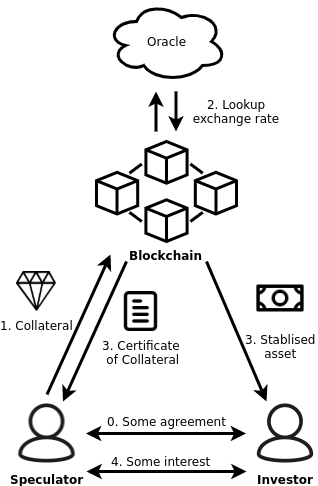
\includegraphics{img/CDP_create.png}
\caption{Stablecoin minting through debt creation
\label{cdp_destroy_label}}
\end{figure}

Figure \ref{cdp_destroy_label} describes the process of minting a
decentralised stablecoin that uses the swap mechanic:

\begin{enumerate}
\def\labelenumi{\arabic{enumi}.}
\setcounter{enumi}{-1}
\tightlist
\item
  Some agreement is reached between the investor and the speculator.
  This might happen on an individual basis, but sometimes the terms of
  the agreement are pre-defined by parameters of the network.
\item
  Some crypto, lets say Ether, is sent as collateral to a
  smart-contract. Some of this, usually 100\%, might come from the
  investor, white the speculator provides the rest of the collateral,
  lets say 50\%, for the stablecoin to remain overcollateralized by some
  ratio, in this case 150\%.
\item
  A smart-contract checks the price of the Ether in terms of the pegged
  currency, lets say dollars. Mechanisms for the decentralised lookup of
  Ether prices vary between systems. We explore these differences later
  in this section.
\item
  The stablecoin is minted and issued to the investor, while the
  speculator gets some proof of deposit for their collateral. Lets call
  this the debt-contract.
\item
  Some interest might be payed from the investor to the speculator or
  vise versa.
\end{enumerate}

The investor might pay interest to the speculator as a reward for
providing the capital for overcollateralization and taking on the risk
of the collateral dropping in value while the stablecoin is in
circulation. On the other hand, the speculator might pay the investor as
a reward for providing extra capital for the speculator to leverage
their bet on Ether. The direction of interest depends on the design of
the stablecoin and sometimes the market conditions.

While the stablecoin is in circulation the speculator is responsible for
maintaining the collateral of debt-contract. Should the value of Ether
drop, they must deposit more Ether to the smart contract, or risk
getting margin called.

A margin call is the automatic closing of a debt contract. A margin call
happens when the value of the collateral drops below the minimum
collateral requirement of the system. In the case of our example this
means there is not enough Ether in the debt-contract to cover 150\% of
the outstanding stablecoins of the contract. A margin call opens the
debt-position to be closed by anyone, and incentivises this by providing
a reward for whoever closes it.

The closing of a contract is the burning of the stablecoin and the
recovery of the underlying collateral. The process for this is
illustrated in figure \label{cdp_destroy_label} and includes the
following steps:

\begin{enumerate}
\def\labelenumi{\arabic{enumi}.}
\setcounter{enumi}{-1}
\tightlist
\item
  Some agreement is reached between an investor willing to sell a
  stablecoin, and a someone willing to close out a debt-contract. This
  agreement could come be in the form of a speculator simply buying the
  coins from an investor at market rate, an investor acting on a margin
  call, or by some other matching mechanism between stablecoin and
  debt-contract.
\item
  The stablecoin is sent to a smart-contract, which burns the coin.
\item
  The oracle is consulted for the current price level of Ether in
  dollars.
\item
  The collateral is provided back to the speculator and investor at some
  defined ratio. Ususally 100\% of the stablecoin value goes to the
  investor while the remaining 50\% or more goes back to the speculator.
\item
  Some settlement may be done, this could be the payment of interest
  between the two parties or some fee to the blockchain.
\end{enumerate}

\begin{figure}
\centering
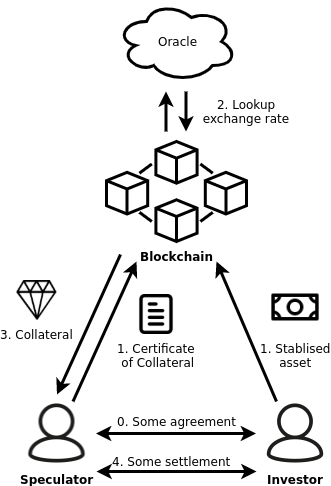
\includegraphics{img/CDP_destroy.png}
\caption{Stablecoin burning through debt-position closage
\label{cdp_destroy_label}}
\end{figure}

As an extra line of defence against the falling of the collateral value
or some attack against the system, crypto-collateralized stablecoins
often have a mechanism for global settlement implemented. In the case of
a global settlement event, the underlying collateral gets returned to
the investors without any conditions. All debt contracts will be locked,
allowing all holders of the stablecoin to trade in their tokens for 1
dollars worth of collateral. After a period of time, the contracts will
be released and return all collateral left back the the speculators.

The triggers for a global settlement differ per stablecoin, but
mechanisms include: global collateralization under a minimum ratio, high
price instability, a decision by holders of some governance token.

\hypertarget{governance}{%
\subsection{Governance}\label{governance}}

In addition to triggering global settlement in the case of some black
swan event, decisions need to be made about the network in general.
Examples of this can be parameter tweaking like the collateralization
ratio or network fees, as well as network upgrades. For this reason most
decentralised stablecoins are part of a Distributed Autonomous
Organisation (DAO). Shares in the DAO, or governance tokens, allow the
holders some say over the inner workings of the network, as well as some
claim of the profits of the network. This ties the value of the tokens
to the to the performance of the network, which in turn incentivises the
holders of the governance tokens to remain invested in the network and
to vote for parameters and mechanisms that improve the utility and
stability of the stablecoin.

\hypertarget{variations-between-stablecoins}{%
\subsection{Variations between
stablecoins}\label{variations-between-stablecoins}}

Multiple stablecoins follow the structure layed-out. The differences can
be expressed in a number of parameters. TODO

\hypertarget{minimum-collateralization-ratio}{%
\subsubsection{Minimum Collateralization
Ratio}\label{minimum-collateralization-ratio}}

The minimum collateral required varies between systems. It is the
responsibility of the speculator to maintain a collateralization ratio
above the minimum requirement, or they get margin called.

The collateralization requirement depends on the volatility of the
collateral used. Since the margin call of a contract takes time to find
an investor someone willing to close it, there needs to be a buffer for
the price of the collateral to fall even further. This buffer is the gap
between the minimum ratio and 100\%.

This means that network doesn't lose any collateral as long as the
collateral doesn't drop to \(1/c\) within the time it takes to margin
call a contract. Where \(c\) is the minimum collateralization ratio.

\hypertarget{mechanism-for-speculator-to-investor-match-making}{%
\subsubsection{Mechanism for speculator to investor match
making}\label{mechanism-for-speculator-to-investor-match-making}}

Stablecoins that utilise these derivative contracts are usually built
with a system that aligns the incentives of the stablecoins within some
structure. Variations in these systems leads to differences in features
like:

\begin{itemize}
\tightlist
\item
  the direction of interest payments,
\item
  the matching of investor to speculator,
\item
  the amount of collateral put up by each party,
\item
  the mechanism of a margin call.
\end{itemize}

To explain the variation between the systems we use some examples. We
show how diffences in the purpose of the system leads to differences in
the features, and how the price keeps stabilising.

\hypertarget{reserve-bank-speculator-model}{%
\paragraph{Reserve bank speculator
model}\label{reserve-bank-speculator-model}}

In the first type of system the speculators collectively act like a
reserve bank.

The creation and destruction of stablecoins are controlled by the
speculator. Anyone can create a debt-contract, deposit collateral and
mint stablecoin tokens as long as they remain properly
overcollateralized. The contract can also be closed at any time by
depositing an equal amount of stablecoins to get the same collateral
back.

It is important to know that, in this system, the amount of stablecoins
created is determined by the price, in say dollars, of the collateral at
the time of minting. This leads to the following incentive structure:

If the market value of the token is higher that 1 dollar a speculator is
incentivised to deposit more collateral and mint more tokens. These
token can then be sold on the market. Increasing the supply, thus
dropping the price back to one dollar. The benefit of the speculator
here is that they were able to create a debt contract at a favorable
rate. If, when they pay back the tokens, the market value of the token
is lower than when they sold the coins, they will make a profit.

If the market value of the token is lower than a dollar, any speculator
with an open contract can buy the tokens at a discount and close their
contract out at a profit given that they bought sold the tokens at a
higher price. This leads to fewer coins on the market, thus increasing
the value back up to a dollar.

This creates a ``soft peg'' as there is no guarantee for the speculator
that when they mint and a coin they will be able to buy it back again at
a lower price. This can lead to the market price of the token rising to
a different price level, and the peg can stabilise at a price level that
is higher or lower than any collateral held.

The price level of the token is thus determined by what the market
believes it is worth. There is some indication however, that the coin
will not drop below 1 dollar, since that is the value that is returned
to investors in the case of margin calls or a global settlement
scenario.

In this scenario, the speculator takes on a certain amount of risk
speculating on the value of the collateral and the price of the token.
Initially it seems like the speculator gets their value from speculation
only. They can, for example, sell their tokens on the market for more of
the collateral thus leveraging their speculation on the collateral by
some factor.

Usually, the designer inteded way for the speculator to make a profit is
by peer to peer lending. Instead of selling the tokens on the market,
the speculator can lend out the tokens to makes some extra dividends
while speculating on the collateral. In this way, the speculator acts as
the reserve bank increasing the supply of the token by lending out more.

Irregardless of how the speculator chooses to use their tokens, anyone
investor buying them has a some guarantee that they will be worth at
least a dollar in the future, thus creating an asset that is more stable
than the underlying collateral.

The complete risk acceptance and decision making of the speculator
allows for a number of expantions on the already explained concepts.
First, since the success of the network is dependent on being properly
collateralized, and this in turn is dependent on the market value of the
collateral, it makes sense to diversify the collateral. Thus, a
multi-collateral system, which improves guarantees for token holders can
be created, where the speculators have a choice in what collateral they
want to stake. This protects the system against a price crash in one
collateral category, as speculators are incentivised to exchange the
collateral that is dropping in value for more price-stable collateral.

\hypertarget{margin-trading}{%
\paragraph{Margin trading}\label{margin-trading}}

in: Speculator: short-sells token, longs collateral, wants more exposure
Investor: seeks stability, longs token pre-set: collateral ratio agree:
on price the investor pays, (hopefully 1 dollar) matches: minimum
offers, maximum interest from speculators matches: maximum offers,
minimum interest from investors

investor: sell token on market speculator: maintain collateral or
margincall

out: speculator: buying back from the market (covering a short)
investor: autoliquidate lowest collateral matches: buy orders from
speculator matches: sell orders from investors

ideal expectation: self-reenforcement of the value

when low: everyone buys bitshares moving the margin up when high:

reality: low demand pushed price down and undercollateralised

interest:

30 day buyback

inflation of shares

\hypertarget{tracker-servicespeculation-market}{%
\paragraph{Tracker service/speculation
market}\label{tracker-servicespeculation-market}}

(Synthetix)

\#\#\#\#To capture:

\begin{itemize}
\tightlist
\item
  Ratio of collateral payed by the investor
\item
  Interest payed from investor to speculator or vice versa
\end{itemize}

\hypertarget{oracles}{%
\subsection{Oracles}\label{oracles}}

\hypertarget{overview}{%
\subsection{Overview}\label{overview}}

\begin{table*}[t]\begin{center}\begin{supertabular}[]{@{}llllllll@{}}
\toprule
\begin{minipage}[b]{0.09\textwidth}\raggedright
Stablecoin\strut
\end{minipage} & \begin{minipage}[b]{0.04\textwidth}\raggedright
Peg\strut
\end{minipage} & \begin{minipage}[b]{0.13\textwidth}\raggedright
Collateral\strut
\end{minipage} & \begin{minipage}[b]{0.06\textwidth}\raggedright
Min. col.\strut
\end{minipage} & \begin{minipage}[b]{0.21\textwidth}\raggedright
Match-making\strut
\end{minipage} & \begin{minipage}[b]{0.11\textwidth}\raggedright
Interest paid\strut
\end{minipage} & \begin{minipage}[b]{0.09\textwidth}\raggedright
Governance\strut
\end{minipage} & \begin{minipage}[b]{0.06\textwidth}\raggedright
Details\strut
\end{minipage}\tabularnewline
\midrule
\begin{minipage}[t]{0.09\textwidth}\raggedright
MakerDAO\strut
\end{minipage} & \begin{minipage}[t]{0.04\textwidth}\raggedright
USD\strut
\end{minipage} & \begin{minipage}[t]{0.13\textwidth}\raggedright
Ether (and more)\strut
\end{minipage} & \begin{minipage}[t]{0.06\textwidth}\raggedright
150\%\strut
\end{minipage} & \begin{minipage}[t]{0.21\textwidth}\raggedright
Speculator to Investor Loan\strut
\end{minipage} & \begin{minipage}[t]{0.11\textwidth}\raggedright
to Speculator\strut
\end{minipage} & \begin{minipage}[t]{0.09\textwidth}\raggedright
\strut
\end{minipage} & \begin{minipage}[t]{0.06\textwidth}\raggedright
\strut
\end{minipage}\tabularnewline
\begin{minipage}[t]{0.09\textwidth}\raggedright
BitShares\strut
\end{minipage} & \begin{minipage}[t]{0.04\textwidth}\raggedright
USD\strut
\end{minipage} & \begin{minipage}[t]{0.13\textwidth}\raggedright
Bitshares\strut
\end{minipage} & \begin{minipage}[t]{0.06\textwidth}\raggedright
300\%\strut
\end{minipage} & \begin{minipage}[t]{0.21\textwidth}\raggedright
Margin Trading\strut
\end{minipage} & \begin{minipage}[t]{0.11\textwidth}\raggedright
to investor\strut
\end{minipage} & \begin{minipage}[t]{0.09\textwidth}\raggedright
\strut
\end{minipage} & \begin{minipage}[t]{0.06\textwidth}\raggedright
\strut
\end{minipage}\tabularnewline
\begin{minipage}[t]{0.09\textwidth}\raggedright
Synthetix\strut
\end{minipage} & \begin{minipage}[t]{0.04\textwidth}\raggedright
USD\strut
\end{minipage} & \begin{minipage}[t]{0.13\textwidth}\raggedright
SNX\strut
\end{minipage} & \begin{minipage}[t]{0.06\textwidth}\raggedright
750\%\strut
\end{minipage} & \begin{minipage}[t]{0.21\textwidth}\raggedright
Global interest calculation\strut
\end{minipage} & \begin{minipage}[t]{0.11\textwidth}\raggedright
\strut
\end{minipage} & \begin{minipage}[t]{0.09\textwidth}\raggedright
\strut
\end{minipage} & \begin{minipage}[t]{0.06\textwidth}\raggedright
\strut
\end{minipage}\tabularnewline
\begin{minipage}[t]{0.09\textwidth}\raggedright
USDQ\strut
\end{minipage} & \begin{minipage}[t]{0.04\textwidth}\raggedright
USD\strut
\end{minipage} & \begin{minipage}[t]{0.13\textwidth}\raggedright
Bitcoin\strut
\end{minipage} & \begin{minipage}[t]{0.06\textwidth}\raggedright
200\%\strut
\end{minipage} & \begin{minipage}[t]{0.21\textwidth}\raggedright
\strut
\end{minipage} & \begin{minipage}[t]{0.11\textwidth}\raggedright
\strut
\end{minipage} & \begin{minipage}[t]{0.09\textwidth}\raggedright
\strut
\end{minipage} & \begin{minipage}[t]{0.06\textwidth}\raggedright
\strut
\end{minipage}\tabularnewline
\bottomrule
\tabularnewline
\end{supertabular}
\caption{TODO \label{TODO}}
\end{center}\end{table*}

To mention: 1. Global settlement 2. Governance 3. Share of collateral,
vs interest 4. BitShares exchange 5. MakerDAO 6. Synthetix 7. Future

\hypertarget{discussions-of-stablecoins}{%
\section{Discussions of Stablecoins}\label{discussions-of-stablecoins}}

Besides the papers describing techniques, some research has been done
into existing stablecoins, quantifying their prevalence, and discussing
their criticisms.

In {[}7{]} Darrel Duffie describes the use of stablecoins for banks
aiming to digitise both inter-organisation value transfer and
governments wanting to implement a digital currency with the utility
benefits of cryptocurrencies and the stability of fiat.

Chohan discusses the difficulties in maintaining a properly
collateralized peg in ``Are Stable Coins Stable?''{[}19{]}. Chohan
describes how maintaining a true 1:1 peg leads to funding and
scalability issues.

In ``The State of Stablecoins''{[}20{]} the ``blockchain team'' present
an empirical study of 57 live and pre-launch stablecoins showing
adoption, trading volume and market cap. They describe a taxonomy where
they differentiate between ``traditional'' collateralized, crypto
collateralized and algorithmic. They describe many pros and cons of
these types of coins. The survey is very extensive and describes all 57
currencies in terms of their investors, tech, legal structure and
collateral format.

In ``Stablecoins in Cryptoeconomics. From Initial Coin Offerings (ICOs)
to Central Bank Digital Currencies''{[}21{]} Erba discusses the
stablecoins in the context of the law in both the united states and
Europe. Erba argues for crypto-currencies ``fully backed by Central Bank
reserves''

In ``Stablecoin: Yet Another Layer of Cryptocurrency
Complexity''{[}22{]} Lee looks at the way that stablecoins can fit into
the modern legal system. Lee argues for Bankruptcy Courts to treat
stablecoins as a commodity as opposed to a currency.

\begin{verbatim}
In [@Fedcoin] Koning describes the requirements and considerations for a stable
currency controlled by a central bank. Koning describes the monetary policy and
choices that comes along with implementing a digital currency on a large scale.
\end{verbatim}

In {[}23{]} Klages-Mundt et al.~look at the existing stablecoins through
a critical lens and describe some ways in which the currency pegs can be
broken. Klages-Mundt build a generalised model of decentralised
crypto-collateralized stablecoins. It describes possible attacks on
these systems where the pegged currency is bid up so an extent where
collateral starts to get margin-called creating a run-away feedback
loop.

\hypertarget{conclusion}{%
\section{Conclusion}\label{conclusion}}

There is a lot happening in the stablecoin and DeFi space right now.
Stablecoins are being tested in a trial by fire in the real-world as we
speak. Through this organisations such as MakerDAO and Synthetix are
developing completely systems that promise to either revolutionise the
world by taking Decentralised Finance to the next level, or they will
spectacularly go up in a ball of fire. Only time will tell.

\hypertarget{references}{%
\section*{References}\label{references}}
\addcontentsline{toc}{section}{References}

\hypertarget{refs}{}
\leavevmode\hypertarget{ref-Money_as_IOUs_in_Social_Trust_Networks}{}%
{[}1{]} R. Fugger, ``Money as ious in social trust networks.''

\leavevmode\hypertarget{ref-TrustChain}{}%
{[}2{]} Martijn de Vos and Johan Pouwelse, ``TrustChain.''
\url{https://repository.tudelft.nl/islandora/object/uuid:c51ac99d-3013-44b3-8ddd-fbd951a2454a}.

\leavevmode\hypertarget{ref-MakerDAO:whitepaper}{}%
{[}3{]} The Maker Team, ``MakerDAO whitepaper.''
\url{https://makerdao.com/whitepaper/DaiDec17WP.pdf}.

\leavevmode\hypertarget{ref-On_the_Origin_of_Money}{}%
{[}4{]} K. Menger, ``On the Origin of Money,'' \emph{The Economic
Journal}, vol. 2, no. 6, pp. 239--255, Jun. 1892.

\leavevmode\hypertarget{ref-Value_of_Money}{}%
{[}5{]} A. C. Pigou, ``The Value of Money,'' \emph{The Quarterly Journal
of Economics}, vol. 32, no. 1, pp. 38--65, Nov. 1917.

\leavevmode\hypertarget{ref-The_Gold_Standard}{}%
{[}6{]} R. N. Cooper, R. Dornbusch, and R. E. Hall, ``The gold standard:
Historical facts and future prospects,'' \emph{Brookings Papers on
Economic Activity}, vol. 1982, no. 1, pp. 1--56, 1982.

\leavevmode\hypertarget{ref-DuffieDigital_and_Fast_Payment_Systems}{}%
{[}7{]} D. Duffie, ``DuffieDigital and fast payment systems.''

\leavevmode\hypertarget{ref-JPMorgan_Coin:whitepaper}{}%
{[}8{]} JPMorgan Chase \& Co., ``J.P.Morgan coin announcement.''
\url{https://www.jpmorgan.com/global/news/digital-coin-payments}.

\leavevmode\hypertarget{ref-Libra:whitepaper}{}%
{[}9{]} ``Libra whitepaper.''
\url{https://libra.org/en-US/white-paper/}.

\leavevmode\hypertarget{ref-Tether:whitepaper}{}%
{[}10{]} Tether International Limited, ``Tether whitepaper.''
\url{https://tether.to/wp-content/uploads/2016/06/TetherWhitePaper.pdf}.

\leavevmode\hypertarget{ref-Centre:whitepaper}{}%
{[}11{]} CENTRE Consortium, ``Centre whitepaper.''
\url{https://www.centre.io/pdfs/centre-whitepaper.pdf}.

\leavevmode\hypertarget{ref-PAXos:whitepaper}{}%
{[}12{]} Charles Cascarilla, ``PAXos whitepaper.''
\url{https://account.paxos.com/whitepaper.pdf}.

\leavevmode\hypertarget{ref-TrueUSD:whitepaper}{}%
{[}13{]} LLC TrueCoin, ``Trust token.''
\url{https://www.trusttoken.com/trueusd}.

\leavevmode\hypertarget{ref-Stasis:whitepaper}{}%
{[}14{]} STASIS Foundation, ``Stasis whitepaper.''
\url{https://stasis.net/}.

\leavevmode\hypertarget{ref-PAXGold:whitepaper}{}%
{[}15{]} Charles Cascarilla, ``PAX gold whitepaper.''
\url{https://www.paxos.com/paxgold/}, 2019.

\leavevmode\hypertarget{ref-DigixDAO:whitepaper}{}%
{[}16{]} Anthony C. Eufemio, ``DigixDAO whitepaper.''
\url{https://digix.global/whitepaper.pdf}.

\leavevmode\hypertarget{ref-globcoin:whitepaper}{}%
{[}17{]} Reserve Currency Solutions, ``Globcoin whitepaper.''
\url{https://globcoin.io/assets/pdf/whitepaper-Globcoin-v3.1.0.pdf}.

\leavevmode\hypertarget{ref-x8currency:whitepaper}{}%
{[}18{]} X8 AG, ``X8currency whitepaper.''
\url{https://x8currency.com/wp-content/uploads/X8-Project-TGE-Whitepaper.pdf}.

\leavevmode\hypertarget{ref-Are_Stable_Coins_Stable}{}%
{[}19{]} U. W. Chohan, ``Are stable coins stable?''

\leavevmode\hypertarget{ref-THE_STATE_OF_STABLECOINS}{}%
{[}20{]} T. B. Team, ``The state of stablecoins.''

\leavevmode\hypertarget{ref-Stablecoins_in_Cryptoeconomics}{}%
{[}21{]} M. Dell'Erba, ``Stablecoins in cryptoeconomics. From initial
coin offerings to central bank digital currencies (cbdcs).''

\leavevmode\hypertarget{ref-Stablecoin:_Yet_Another_Layer_of_Cryptocurrency_Complexity}{}%
{[}22{]} M. Lee, ``Stablecoin: Yet another layer of cryptocurrency
complexity,'' \emph{American Bankruptcy Institute Journal}, vol. 38, no.
9, pp. 36--37, 64, Sep. 2019.

\leavevmode\hypertarget{ref-In_stability_for_the_Blockchain}{}%
{[}23{]} A. M. Ariah Klages-Mundt, ``(In)stability for the blockchain:
Deleveraging spirals and stablecoin attacks.''

\end{document}

